\subsection{Effect of the number of samples in the Kolmogorov-Smirnov validation test} \label{sec:ks_optimization}
As it has been explained in Sections \ref{sec:ks-results} and \ref{sec:autocorrelation_idle_results}, we faced different problems in the Kolmogorov-Smirnov validation test that make us reconsider this test as the proper one to validate our results. It has been demonstrated that even for really low p-values in the \acs{K-S}, the visual fitting of the estimated and empirical idle distributions is almost perfect. In addition, we studied the independence of the idle samples with an autocorrelation study that showed that the samples are independent enough to be used in the validation test. In addition to this, we tested the separation of the samples gathering one sample every three or five samples to increase the independence but the results obtained were the same.

In this section, we studied the effect of the number of samples used in the \acs{K-S} test to perform the validation. The first implementation of the \acs{K-S} test included a 10 \% of the total idle samples to perform the validation test. The decision of using a percentage of the total number of samples was done just to perform the validation test faster. In this experiment, we tested the performance of the test using all the samples and compared against the first implementation in order to observe if a higher number of samples has an impact in the validation test.

We simulated 100 runs of the same traffic configuration for the session and flow levels, randomizing the packet level as it has been done previously. The traffic configuration for this experiment is presented in Table \ref{table:KS_traffic} in Section \ref{sec:ks-results}. We used three different packet interarrival distributions as it has been done to obtain the results in \ref{table:KS} and extracted the D and P values of the \acs{K-S} test. 

We compared the results obtained between both \acs{K-S} implementations. The results of this experiment are presented in Figure \ref{fig:ks_optimization}. We represented the CDF of the p-value of the \acs{K-S} for 100 runs of each test and compare the performance of the p-value using different number of samples for the validation test. As it can be observed, the performance of the validation test is highly improved using all the samples for the estimation of the p-value. Table \ref{table:KS_optimized} includes a resume of the three cases under study in Table \ref{table:KS} and compared with the \acs{K-S} performance using all the samples.

\begin{figure}[h!]
	\centering
		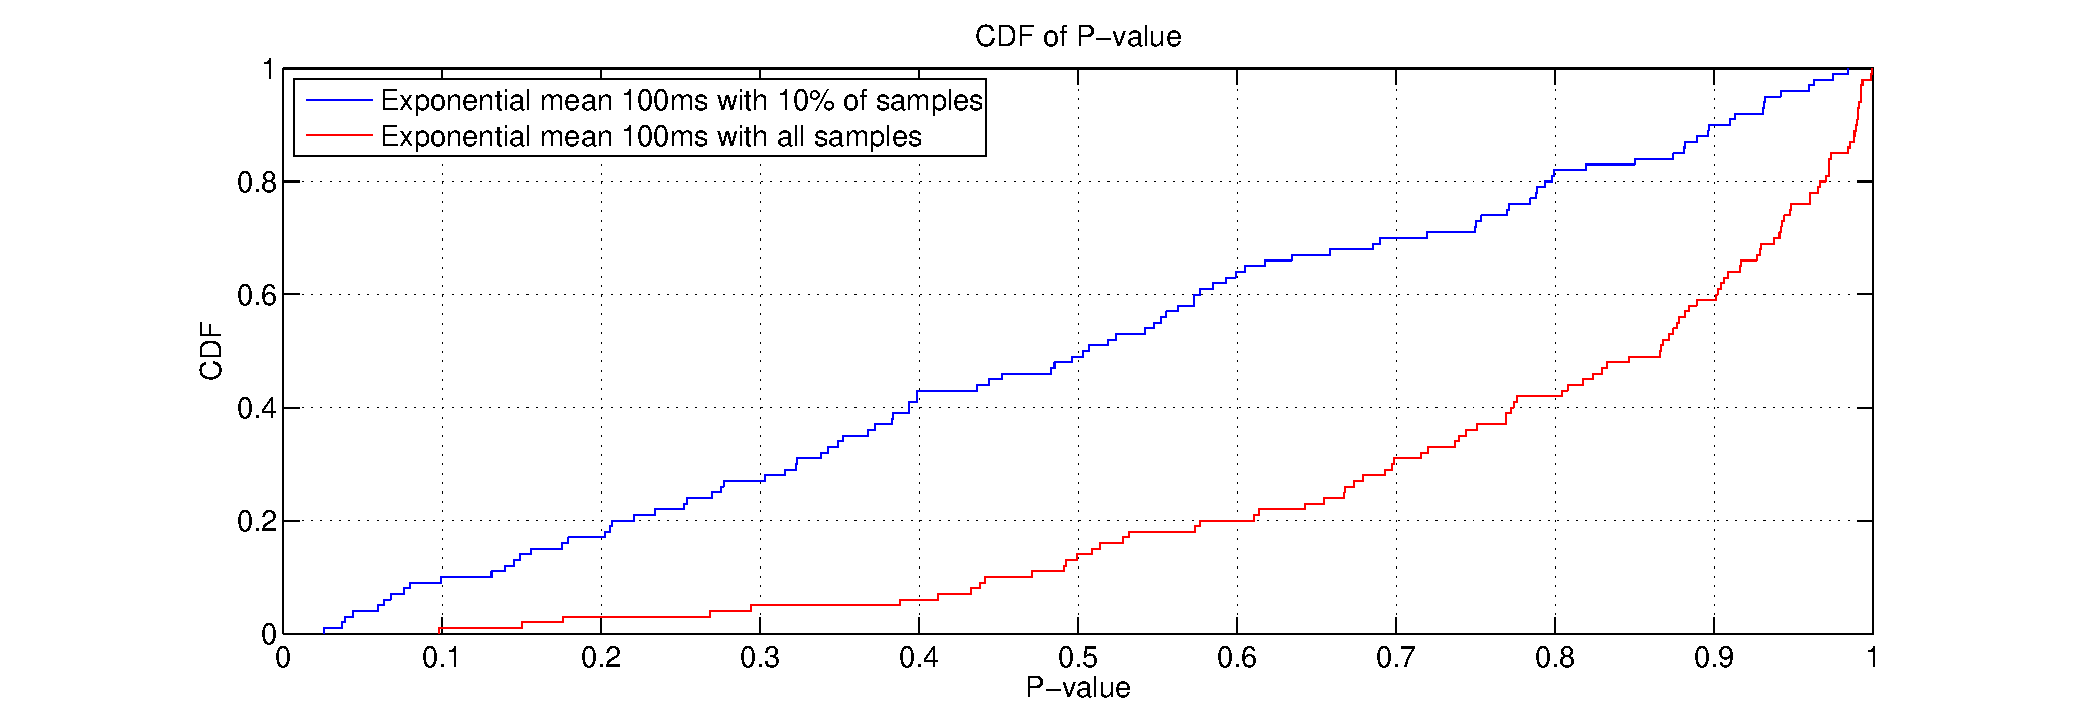
\includegraphics[width=\textwidth, trim = 0mm 0mm 0mm 0mm, clip]{images/results/GlobalView/KS/ks_optimization/pvalue_exponential100ms}
		\label{fig:ks_optimization_exp100}
	\caption{P-value failure rate in the \acs{K-S} test using different number of samples. Exponential packet interarrival with mean 100 ms}
	\label{fig:ks_optimization}
\end{figure}

\begin{table}[h!]
	\centering
	\begin{tabular}{ r | c | c }
		& \acs{K-S} with 10\% of samples & \acs{K-S} with all the samples \\ \hline
		Exponential Interarrival (mean: 1000 ms) & 11.34\% & 0\% \\ 
		Exponential Interarrival (mean: 100 ms) & 10\% & 1\% \\ 
		Uniform Interarrival (mean: 100 ms) & 10.989\% & 10.101\% \\ 
	\end{tabular}
	\caption{\acs{K-S} performance for different packet interarrival distributions and uniform packet size with mean 1550 bytes.}
	\label{table:KS_optimized}
\end{table}

As it can be observed from the statistics presented in Table \ref{table:KS_optimized} the failure rate ($P(P-value<0.1)$) is clearly improved, and almost null for the exponential cases under study in Section \ref{sec:ks-results}. On the other hand, that improvement is not that clear in the uniform distribution.

Using a percentage of all the samples for the validation test, it is possible that the firsts and tail samples are excluded from the set of samples that will be used to estimate the p-value of the \acs{K-S} test affecting the final performance of the validation test. This problem is avoided by using all the set of samples for the validation test and achieving a higher accuracy as it has been demonstrated in this experiment. On the other hand, a higher number of samples implies a higher execution time.

From the results presented in this section, we can conclude that the \acs{K-S} is the correct validation test to be used for our model if all the samples gathered for the estimation of the parameters are also used for the validation test. Using all the idle samples for the validation test we achieve a better performance and avoid the problems presented in Sections \ref{sec:ks-results} and \ref{sec:autocorrelation_idle_results}.